%-------------------------------------------------------------------------------------------------%
% Author: John Joseph Valletta
% Date: 04/03/2015
% Title: Classification
%-------------------------------------------------------------------------------------------------%
% Preamble
\documentclass[pdf]{beamer}
\usepackage{textpos} % for logo placement in headline
\usepackage[export]{adjustbox}
\usepackage{framed}
%-------------------------------------------------------------------------------------------------%
\newif\ifplacelogo % Create a new conditional to avoid displaying logo on every slide
\placelogotrue % Set it to true
\mode<presentation>{\usetheme{Madrid}} % default Antibes Berlin Madrid Montpelier Ilmenau CambridgeUS Berkeley Singapore Copenhagen Malmoe Warsaw
\usecolortheme{dolphin}
\useinnertheme{circles} % circles, rectanges, rounded, inmargin
\usefonttheme[onlymath]{serif} % Makes math fonts like the usual LaTeX ones
%\useoutertheme{tree} % infolines, smoothbars, sidebar, split, tree
\setbeamercovered{transparent=5} % Transparent 10% overlays
\setbeamertemplate{caption}{\raggedright\insertcaption\par} % Remove the word "Figure" from caption %\setbeamertemplate{caption}[default]
\setbeamertemplate{navigation symbols}{} % don't put navigation tools at the bottom (alternatively \beamertemplatenavigationsymbolsempty)
\graphicspath{ {./Figures/} }

% Titlepage
\title{Practical Issues}
\subtitle{or avoiding machine learning going mad}
\author{John Joseph Valletta}
\date[1st-2nd June 2015]{1st-2nd June 2015}
\institute[Penryn Campus]{University of Exeter, Penryn Campus, UK}
% \logo{
%   \makebox[0.95\paperwidth]{
%     
\includegraphics[width=4cm,keepaspectratio]{logo1.pdf}
%     \hfill
%     
\includegraphics[width=4cm,keepaspectratio]{logo2.pdf}
%   }
% }
% Logo
\logo{\ifplacelogo
\includegraphics[width=4cm,keepaspectratio, left]{logo2.pdf}\fi}
\addtobeamertemplate{headline}{}{\ifplacelogo
\begin{textblock*}{100mm}(.68\textwidth,+0.1cm)%.015 instead of 0.68 originally

\includegraphics[width=4cm,keepaspectratio]{logo1.pdf}
\end{textblock*}\fi}
%\author{John Joseph Valletta, Alex Thornton and Mario Recker}
%-------------------------------------------------------------------------------------------------%
% Start of Document
%-------------------------------------------------------------------------------------------------%
\begin{document}
%-------------------------------------------------------------------------------------------------%
\begin{frame}
\titlepage
\end{frame}
\placelogofalse % Turn logo off
%-------------------------------------------------------------------------------------------------%
\begin{frame}{Overview}
\begin{itemize}\addtolength{\itemsep}{0.5\baselineskip}
	\item<2-> Machine learning gone mad
	\item<3-> Laws of data analysis
 	\item<4-> A few important tips
	\item<5-> Which machine learning algorithm should I use?
	\item<6-> Validating models
\end{itemize}
\end{frame}
%-------------------------------------------------------------------------------------------------%
\begin{frame}{Machine learning gone mad - The US tank experiment}
\begin{itemize}\addtolength{\itemsep}{0.5\baselineskip}
	\item<1-> 1980s: Pentagon got excited about artificial neural networks
	\item<2-> Wanted a classifier to detect whether a tank is hiding behind trees
	\item<3-> Collected photos of trees with/without tanks hiding in them
	\item<4-> Trained neural network performed \textit{excellently} on the testing dataset\\
	\textbf{Champagne to all the scientists!}
\end{itemize}
\begin{center}
		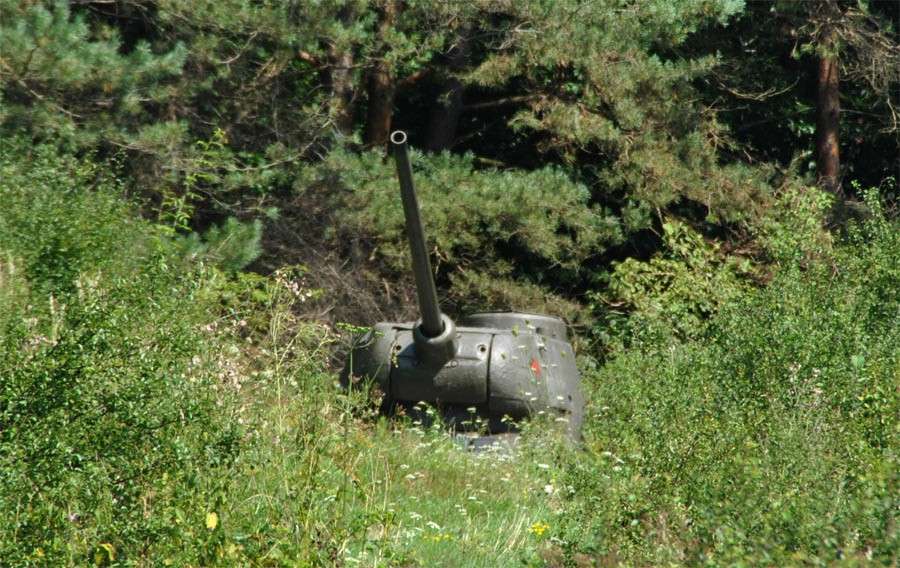
\includegraphics[width=0.5\textwidth]{tank.jpg}
\end{center}
\end{frame}
%-------------------------------------------------------------------------------------------------%
\begin{frame}{Machine learning gone mad - The US tank experiment}
\begin{itemize}\addtolength{\itemsep}{0.5\baselineskip}
	\item<1-> Another set of tank/no tank photos was commissioned
	\item<2-> The classifier was now useless and no better than randomly guessing
	\item<3-> Someone then noted the following on the original dataset:
	\begin{description}[no tank:]
		\item[no tank:] \textit{all} photos taken on a sunny, \textbf{blue} skies day
		\item[tank:] \textit{all} photos taken on a cloudy, \textbf{grey} skies day
	\end{description}
	\item<4-> Neural network had learnt whether it was a sunny or cloudy day\\
	\textbf{God bless the United States of America!}
\end{itemize}	
\begin{center}
		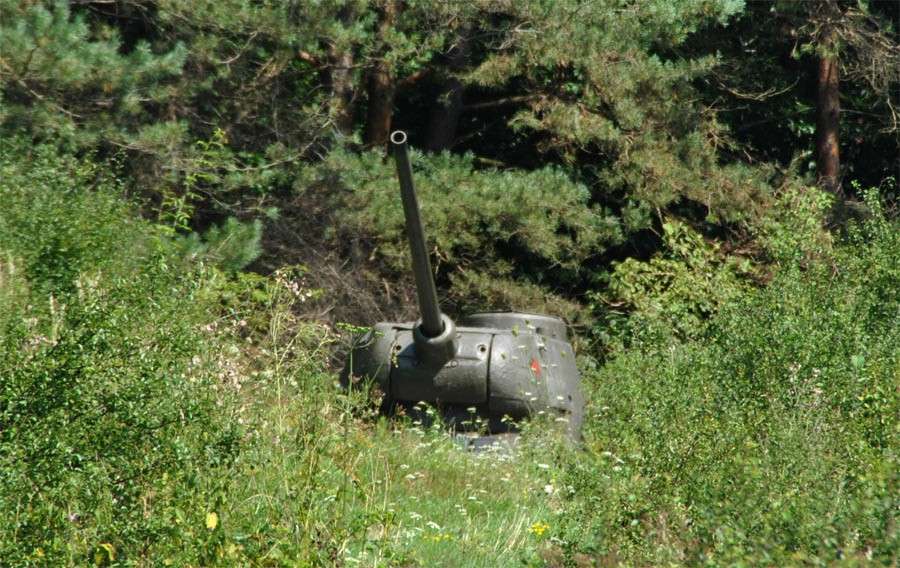
\includegraphics[width=0.5\textwidth]{tank.jpg}
\end{center}
\end{frame}	
%-------------------------------------------------------------------------------------------------%
\begin{frame}{Machine learning gone mad - Google flu trends}
\begin{itemize}\addtolength{\itemsep}{0.5\baselineskip}
	\item<1-> 2008: Google decided to showcase the power of big data 
	\item<2-> Wanted a predictive model to estimate influenza activity	
	\item<3-> Training data were queries containing terms such as cough and fever
	\item<4-> Used IP address to break data by states
	\item<5-> Outcome (label) was influenza-like illness (ILI) physician visits collected by CDC 
	(Centers for Disease Control and Prevention)
	\item<6-> Model was successful, it predicted a spike in the mid-Atlantic region of the US two weeks prior to the CDC\\
	\textbf{Google is great!}
\end{itemize}
\end{frame}
%-------------------------------------------------------------------------------------------------%
\begin{frame}{Machine learning gone mad - Google flu trends}
\begin{center}
		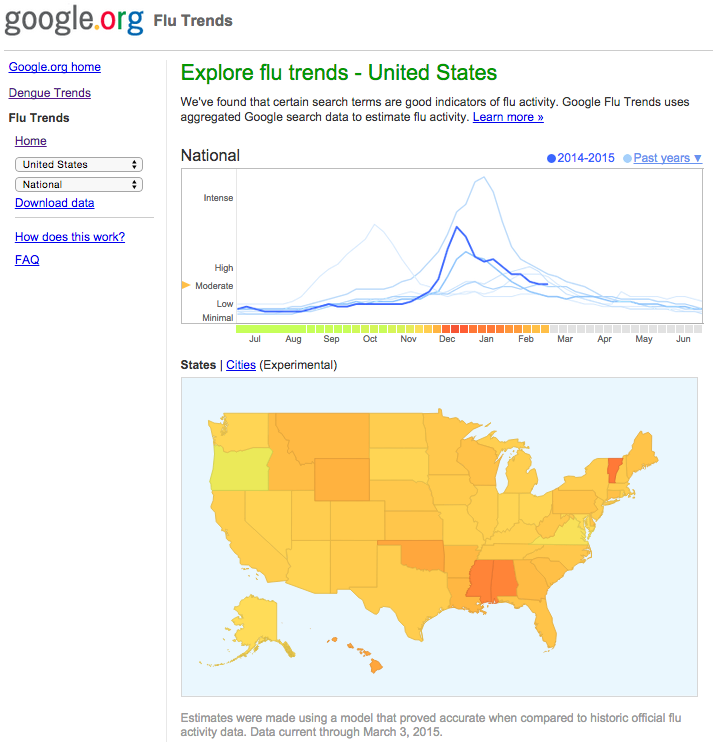
\includegraphics[width=0.65\textwidth]{googleFluTrend1.png}
\end{center}
\end{frame}
%-------------------------------------------------------------------------------------------------%
\begin{frame}{Machine learning gone mad - Google flu trends}
\begin{center}
		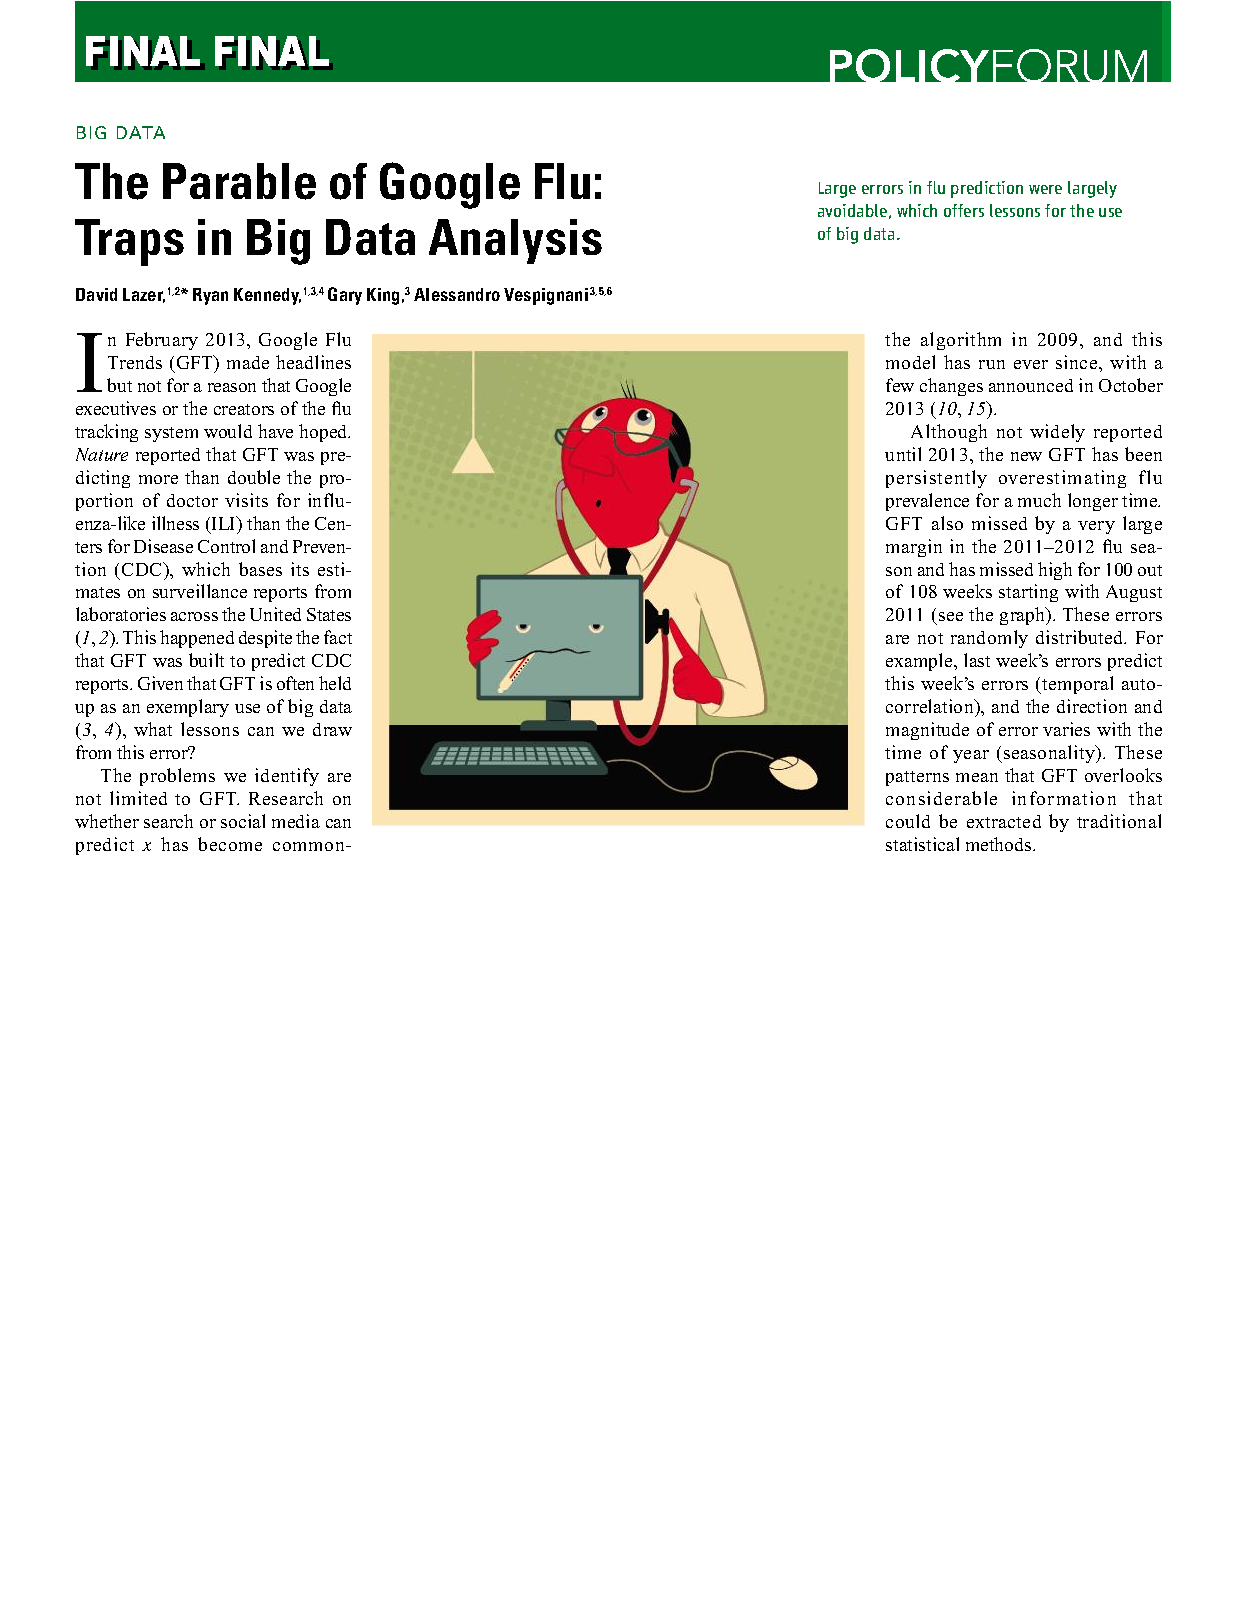
\includegraphics[width=0.85\textwidth]{googleFluTrend2.pdf}
\end{center}
\end{frame}
%-------------------------------------------------------------------------------------------------%
\begin{frame}{Machine learning gone mad - Google flu trends}
\begin{center}
		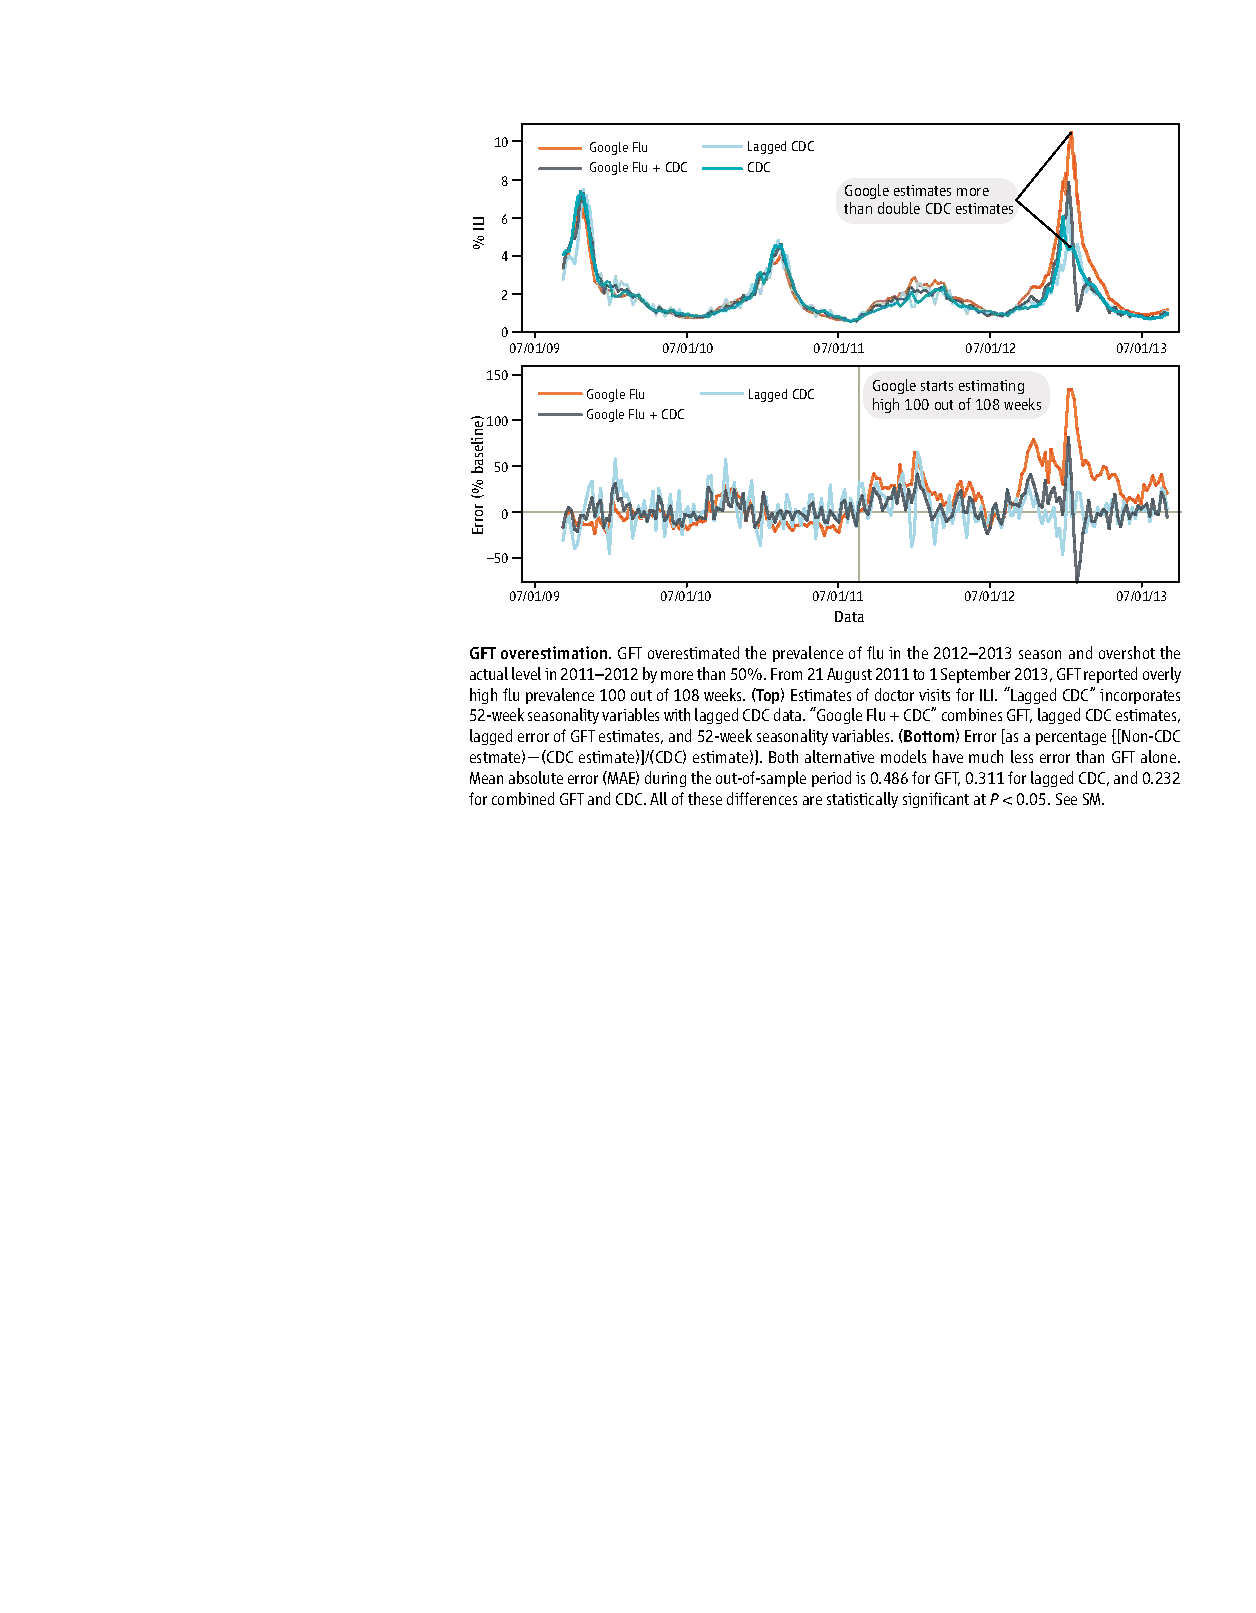
\includegraphics[width=0.7\textwidth]{googleFluTrend3.pdf}
\end{center}
\end{frame}
%-------------------------------------------------------------------------------------------------%
\begin{frame}{Google flu trends, so what went wrong?}
\begin{itemize}\addtolength{\itemsep}{0.5\baselineskip}
	\item<1-> Google had to mine 50 million search terms that best correlated with 1,152 ``true'' data points 
	collected by CDC (Centers for Disease Control and Prevention). They retained 45 queries 
	\item<2-> Winter is coming: Correlation is not causation
	\item<3-> Are these correlates stable and comparable over time?
	\item<4-> Google's search algorithm changes very frequently. Autosuggest feature might have implicitly 
	caused more people to search flu-related terms 
	\item<5-> Is it time to recalibrate the model and/or hybridise both data sources?
	\item<6-> In 2014, Google retrained and updated the model significantly\\ 
	\textbf{Will wait and see!}
\end{itemize}
\end{frame}
%-------------------------------------------------------------------------------------------------%
\begin{frame}{Laws of data analysis}
\begin{enumerate}\addtolength{\itemsep}{1.5\baselineskip}
	\item<2-> Shite in, shite out\\
			\textit{Anonymous}
	\item<3-> If you torture the data long enough it will confess to anything\\
			\textit{Ronald Coase} (1910 - 2013)
	\item<4-> A sufficiently elaborate analysis process can always lend an air of legitimacy\\ 
			\textit{Chris Laws, ex-McLaren boss} 
\end{enumerate}
\end{frame}
%-------------------------------------------------------------------------------------------------%
\begin{frame}{A few important tips}
\begin{itemize}\addtolength{\itemsep}{0.4\baselineskip}
	\item \textbf{Data exploration} can reveal important characteristics in the data\\ 
	e.g histograms, boxplots, scatter plot matrix (plot your raw data!)
	\item Covariates with \textbf{little variability} should be discarded
	\item How are the predictors \textbf{correlated} to each other? 
	\item Missing data - ignore or \textbf{impute}?
	\item \textbf{Standardise} or \textbf{normalise} predictors with widely varying ranges
	\item \textbf{Features} extracted from data are \textbf{key}, they need to be directly relevant to the question
	you're asking
	\item Use \textbf{expert application knowledge} over automatic feature extraction 
	\item \textbf{Never} trust predictions for inputs outside the training dataset range 
	(i.e avoid extrapolation)
\end{itemize}
\end{frame}
%-------------------------------------------------------------------------------------------------%
\begin{frame}{Which machine learning algorithm should I use?}
 \begin{itemize}\addtolength{\itemsep}{0.8\baselineskip}
	\item A personal choice/what you're comfortable using rather than some rules set in stone
	\item Always start with simple models before using more complex ones
	\item Some methods are more appropriate than others in certain domains:
\end{itemize}
\vfill
\small
\begin{description}
		\item [Interpretability:] Decision trees or association rule learning
		\item [Lots of independent features and data:] Na\"{i}ve bayes
		\item [Knowledge of which features are correlated with each other:] Bayesian network
		\item [Thousands of mixed categorical and continuous variables:] Random forests
\end{description}
\normalsize
\end{frame}
%-------------------------------------------------------------------------------------------------%
\begin{frame}{Which machine learning algorithm should I use?}
\begin{figure}	
	\begin{center}
		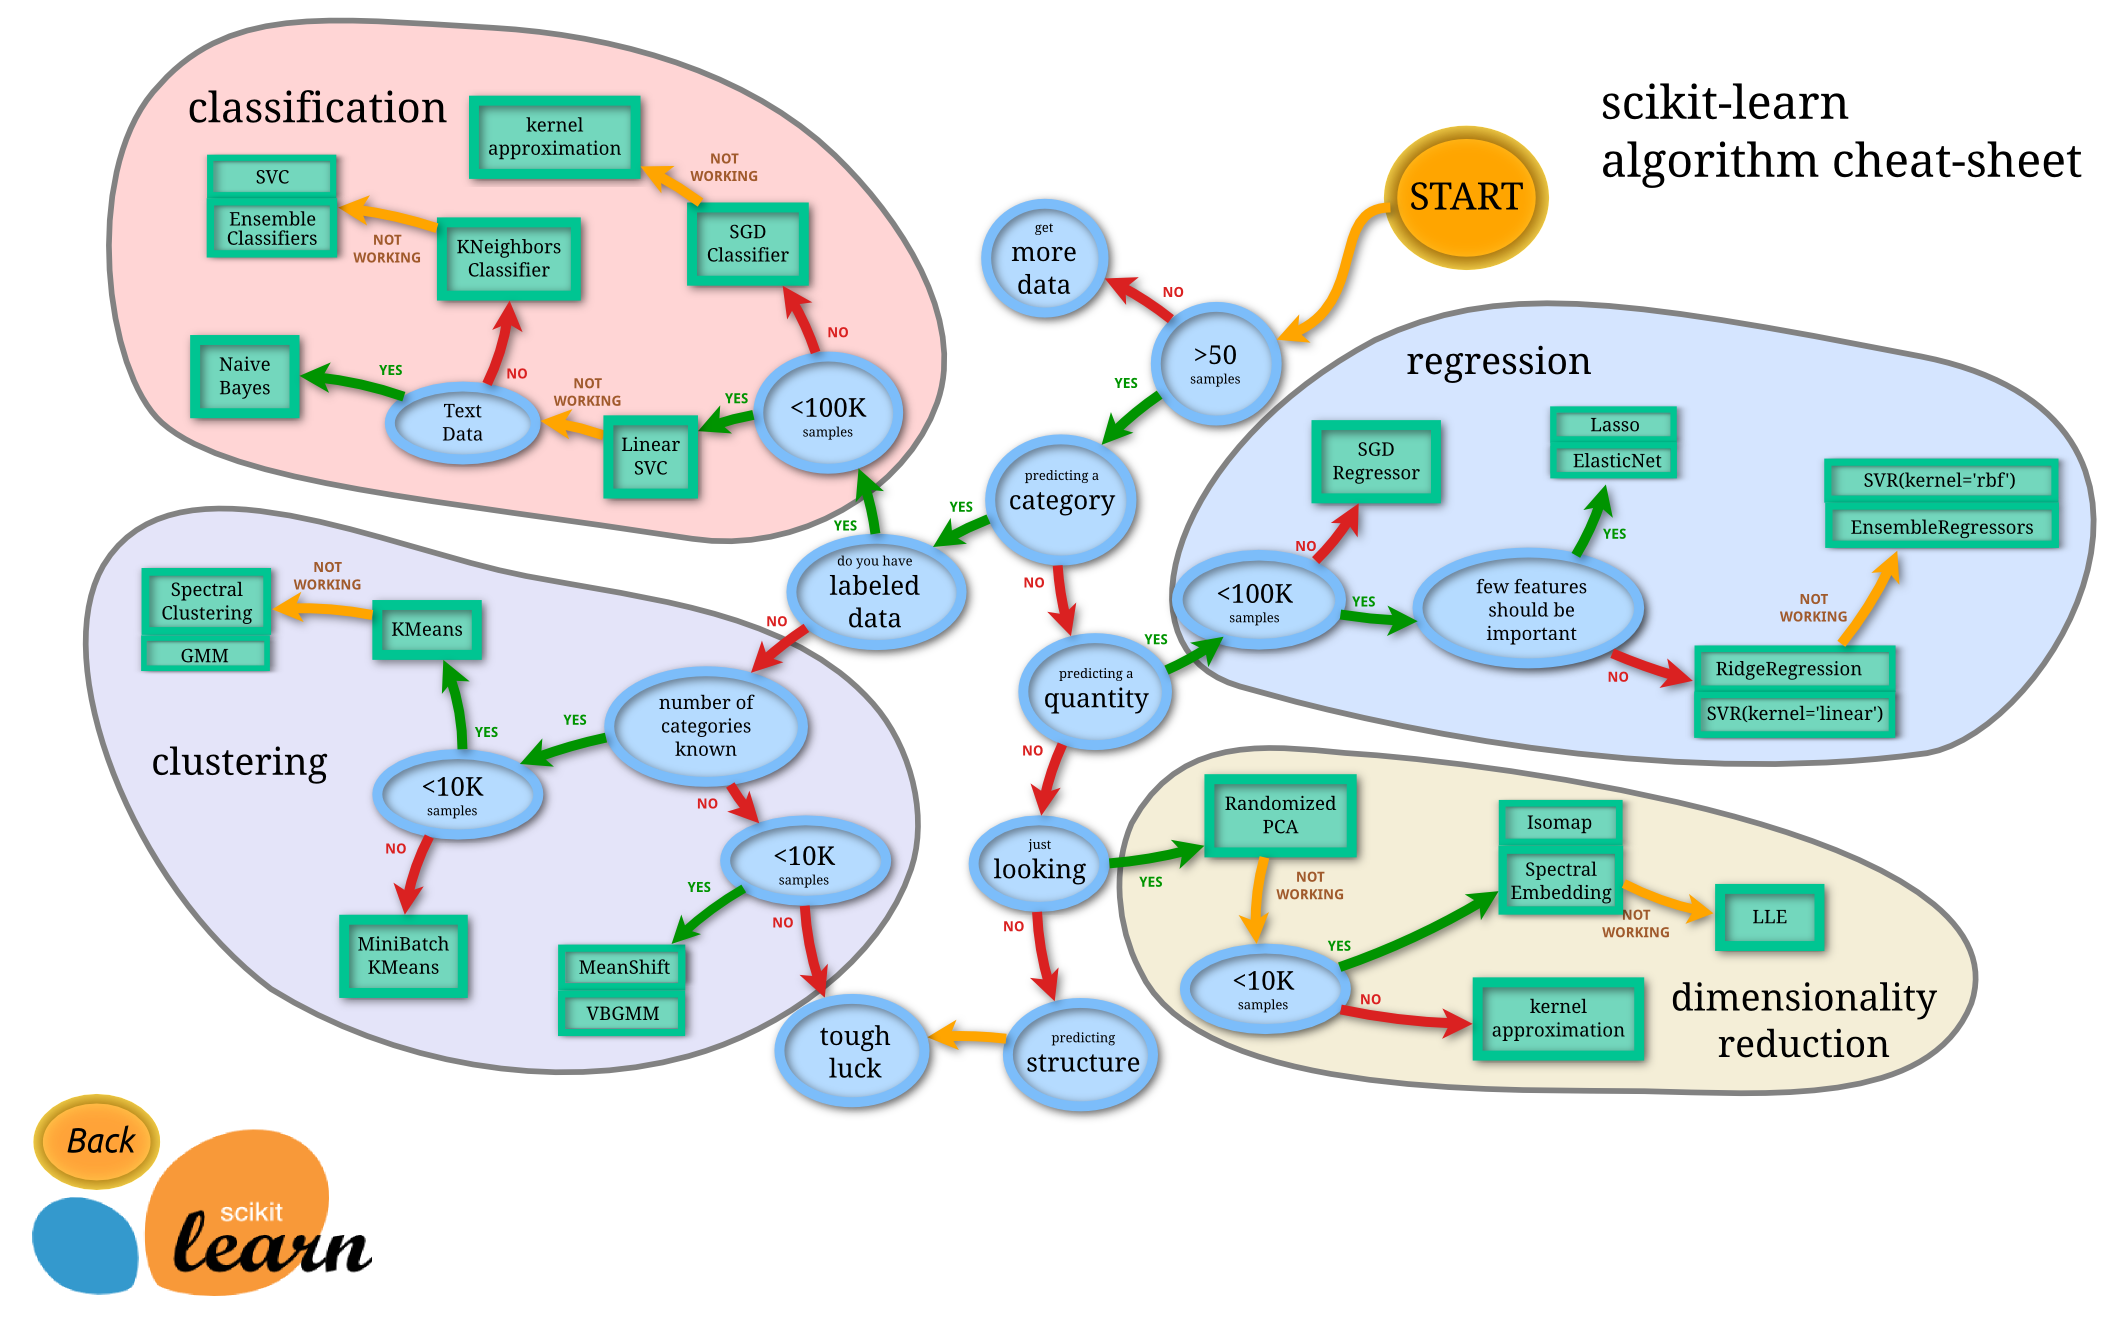
\includegraphics[width=0.98\textwidth]{scikitFlowChart.png}
		\caption{Source: \href{http://scikit-learn.org/stable/tutorial/machine_learning_map/index.html}{scikit-learn.org}}
	\end{center}
\end{figure}
\end{frame}
%-------------------------------------------------------------------------------------------------%
\begin{frame}{Selecting and validating models}
Recall the bias-–variance tradeoff:
\vfill
\begin{center}
	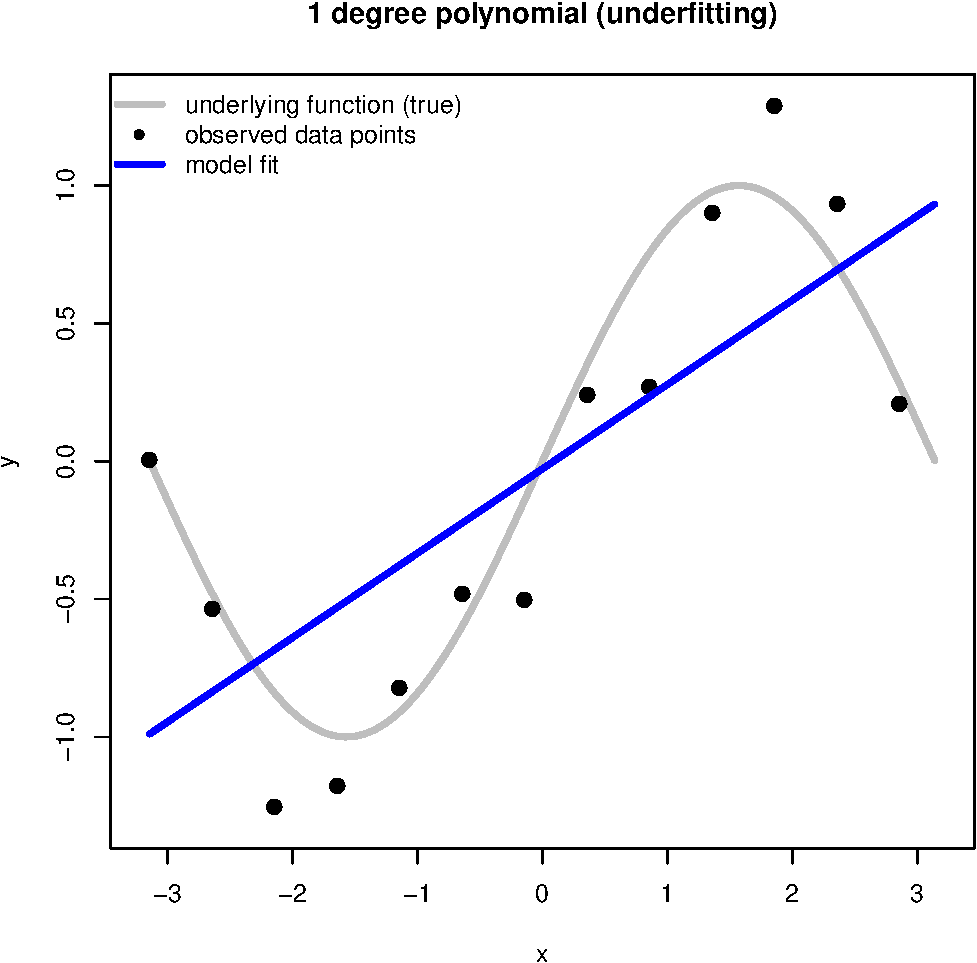
\includegraphics[width=0.333\textwidth]{polyFit1.pdf}
	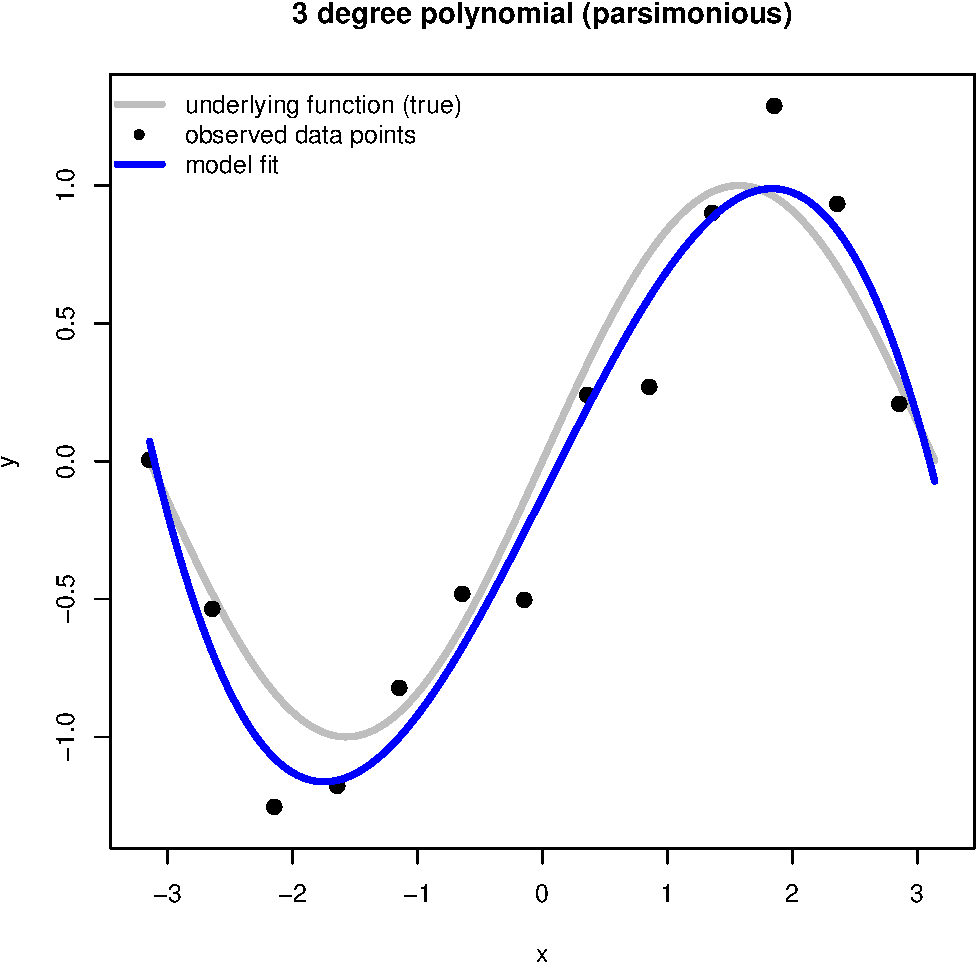
\includegraphics[width=0.333\textwidth]{polyFit3.pdf}
	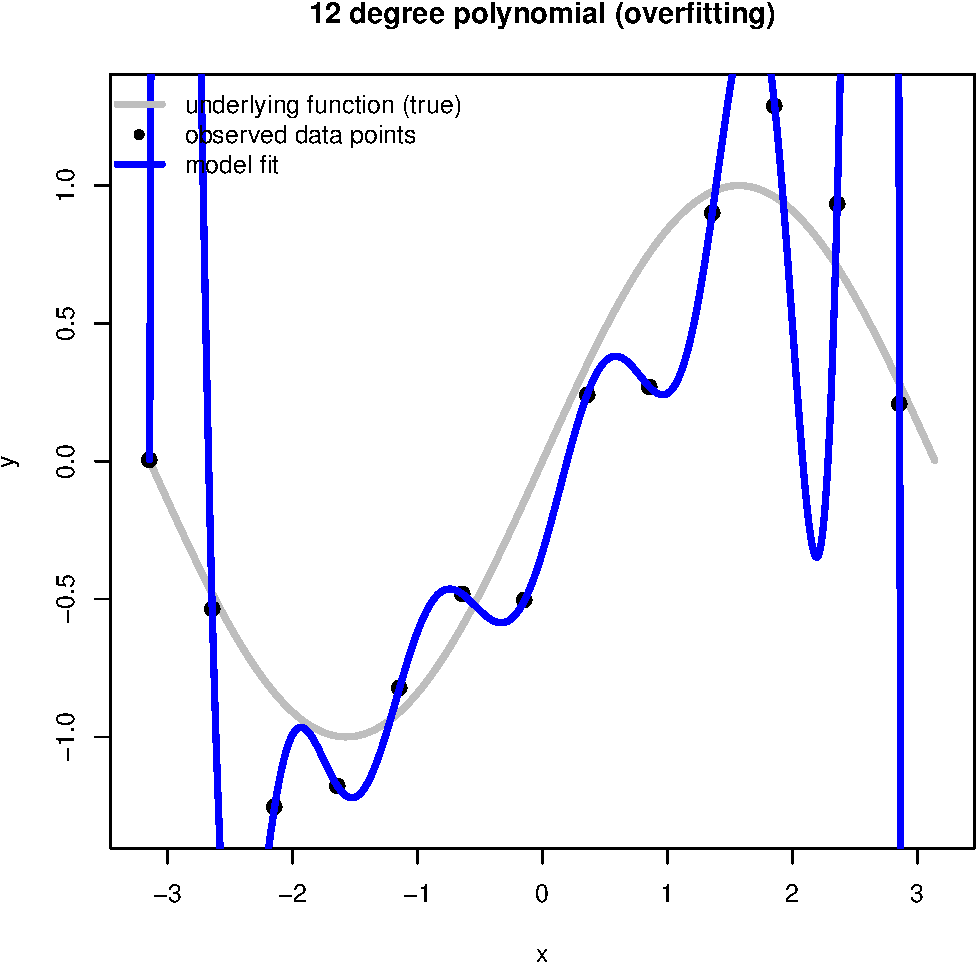
\includegraphics[width=0.333\textwidth]{polyFit12.pdf}
\end{center}
\vfill
\textbf{How do we choose model complexity (model selection)?}\\
\textbf{Once we choose it, how do we validate/assess it?}
\end{frame}
%-------------------------------------------------------------------------------------------------%
\begin{frame}{Selecting and validating models}
\begin{itemize}
	\item<1-> Split data into three parts:
	\begin{center}
		\includegraphics<1->[width=0.5\textwidth]{datasets.png}
		\\
		\visible<2->{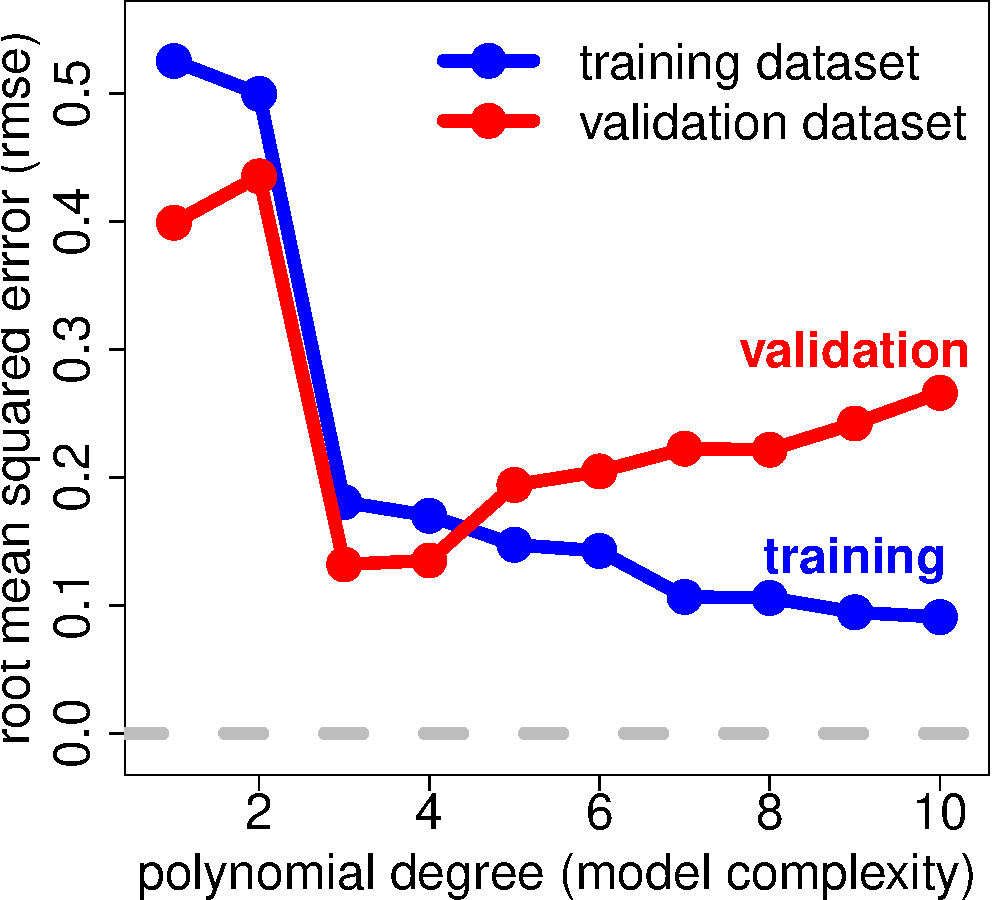
\includegraphics[width=0.5\textwidth]{trainvsval.pdf}}
	\end{center}
\end{itemize}
\end{frame}
%-------------------------------------------------------------------------------------------------%
\begin{frame}{Selecting and validating models}
\begin{itemize}
	\item<1-> When data is limited use $k$-fold cross-validation to estimate test error
	\vfill
	\begin{center}
		\includegraphics<1->[width=0.4\textwidth]{crossvalidation.png}
	\end{center}
\end{itemize}
\visible<2->{\begin{framed}
\vfill
\textbf{Remember}: the most rigorous assessment is to apply the model to an ``unseen'' dataset
\end{framed}}
\end{frame}
%-------------------------------------------------------------------------------------------------%
\end{document}
%-------------------------------------------------------------------------------------------------%
% End of Document
%-------------------------------------------------------------------------------------------------%